\PassOptionsToPackage{unicode=true}{hyperref} % options for packages loaded elsewhere
\PassOptionsToPackage{hyphens}{url}
\documentclass[11pt,ignorenonframetext,aspectratio=169]{beamer}
\IfFileExists{pgfpages.sty}{\usepackage{pgfpages}}{}
\setbeamertemplate{caption}[numbered]
\setbeamertemplate{caption label separator}{: }
\setbeamercolor{caption name}{fg=normal text.fg}
\beamertemplatenavigationsymbolsempty
\usepackage{lmodern}
\usepackage{amssymb,amsmath}
\usepackage{ifxetex,ifluatex}
\usepackage{fixltx2e} % provides \textsubscript
\ifnum 0\ifxetex 1\fi\ifluatex 1\fi=0 % if pdftex
  \usepackage[T1]{fontenc}
  \usepackage[utf8]{inputenc}
\else % if luatex or xelatex
  \ifxetex
    \usepackage{mathspec}
  \else
    \usepackage{fontspec}
\fi
\defaultfontfeatures{Ligatures=TeX,Scale=MatchLowercase}







\fi

  \usetheme[]{metropolis}






% use upquote if available, for straight quotes in verbatim environments
\IfFileExists{upquote.sty}{\usepackage{upquote}}{}
% use microtype if available
\IfFileExists{microtype.sty}{%
  \usepackage{microtype}
  \UseMicrotypeSet[protrusion]{basicmath} % disable protrusion for tt fonts
}{}


\newif\ifbibliography
  \usepackage[round]{natbib}
  \bibliographystyle{plainnat}


\hypersetup{
      pdftitle={Selection in self pollinated crops},
        pdfauthor={Deependra Dhakal},
          pdfborder={0 0 0},
    breaklinks=true}
%\urlstyle{same}  % Use monospace font for urls







% Prevent slide breaks in the middle of a paragraph:
\widowpenalties 1 10000
\raggedbottom

  \AtBeginPart{
    \let\insertpartnumber\relax
    \let\partname\relax
    \frame{\partpage}
  }
  \AtBeginSection{
    \ifbibliography
    \else
      \let\insertsectionnumber\relax
      \let\sectionname\relax
      \frame{\sectionpage}
    \fi
  }
  \AtBeginSubsection{
    \let\insertsubsectionnumber\relax
    \let\subsectionname\relax
    \frame{\subsectionpage}
  }



\setlength{\parindent}{0pt}
\setlength{\parskip}{6pt plus 2pt minus 1pt}
\setlength{\emergencystretch}{3em}  % prevent overfull lines
\providecommand{\tightlist}{%
  \setlength{\itemsep}{0pt}\setlength{\parskip}{0pt}}

  \setcounter{secnumdepth}{0}


  \usepackage{setspace}
  \usepackage{wasysym}
  % \usepackage{fontenc}
  \usepackage{booktabs,siunitx}
  \usepackage{longtable}
  \usepackage{array}
  \usepackage{multirow}
  \usepackage{wrapfig}
  \usepackage{float}
  \usepackage{colortbl}
  \usepackage{pdflscape}
  \usepackage{tabu}
  \usepackage{threeparttable}
  \usepackage{threeparttablex}
  \usepackage[normalem]{ulem}
  \usepackage{makecell}
  \usepackage{xcolor}
  \usepackage{tikz} % required for image opacity change
  \usepackage[absolute,overlay]{textpos} % for text formatting
  \usepackage[skip=0.333\baselineskip]{caption}
  % \usepackage{newtxtext,newtxmath}% better than txfonts   
  \usepackage[english]{babel}
  \usepackage{pgfpages}

  \sisetup{per-mode=symbol}

  % % Added by CII
  % \usepackage[format=hang,labelfont=bf,margin=0.5cm,justification=centering]{caption}
  % \captionsetup{font=small,width=0.9\linewidth,labelfont=small,textfont={small}}
  % % End of CII addition

  % \usepackage{subcaption}
  % \newcommand{\subfloat}[2][need a sub-caption]{\subcaptionbox{#1}{#2}}

  \captionsetup[sub]{font=footnotesize,labelfont=footnotesize,textfont=footnotesize}
  % \captionsetup[subfigure]{font=small,labelfont=small,textfont=small}
  % \captionsetup[subfloat]{font=scriptsize,labelfont=scriptsize,textfont=scriptsize}

  % this font option is amenable for beamer, although these are global settings
  \setbeamerfont{caption}{size=\tiny}
  % \setbeamerfont{subcaption}{size=\tiny} % this does not chage subfloat fonts
  % \setbeamerfont{subfloat}{size=\tiny} % this does not change subfloat fonts
   
   % use single line spacing ?
  \singlespacing

  % use cslreferences environment
  % this is revised as of Oct, 2022 (https://stackoverflow.com/questions/59193797/pandocs-environment-cslreferences-undefined-when-knitting-rmarkdown-to-pdf-in-r)
  \newlength{\cslhangindent}
  \setlength{\cslhangindent}{1.5em}
  \newenvironment{CSLReferences}%
    {\setlength{\parindent}{0pt}%
    \everypar{\setlength{\hangindent}{\cslhangindent}}\ignorespaces}%
    {\par}


  \newcommand{\bcolumns}{\begin{columns}[T, onlytextwidth]}
  \newcommand{\ecolumns}{\end{columns}}

  \newcommand{\bdescription}{\begin{description}}
  \newcommand{\edescription}{\end{description}}

  \newcommand{\bitemize}{\begin{itemize}}
  \newcommand{\eitemize}{\end{itemize}}

  \title[]{Selection in self pollinated crops}


  \author[
        Deependra Dhakal
    ]{Deependra Dhakal}

  \institute[
    ]{
    Agriculture and Forestry University\\
\textit{ddhakal.rookie@gmail.com}\\
\url{https://rookie.rbind.io}
    }

\date[
      
  ]{
    }


\begin{document}

% Hide progress bar and footline on titlepage
  \begin{frame}[plain]
  \titlepage
  \end{frame}



\hypertarget{introduction}{%
\section{Introduction}\label{introduction}}

\begin{frame}{}
\protect\hypertarget{section}{}
\begin{figure}
  \begin{columns}[T,onlytextwidth,c]
  \column{.3\linewidth}
  \begin{quote}
  \footnotesize
  The feet are the wheels of the brain.
  \end{quote}
  \scriptsize \hfill\raggedright -- Herbert Simon (1916-2001) (Political Scientist)
  \column{.5\linewidth}
  \begin{center}
  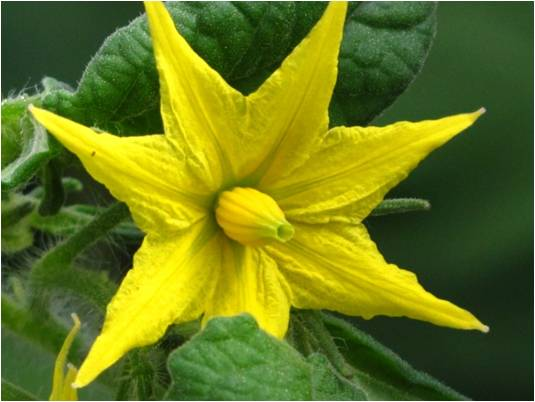
\includegraphics[width=0.65\linewidth]{./images/self_tomato_flower.jpg}
  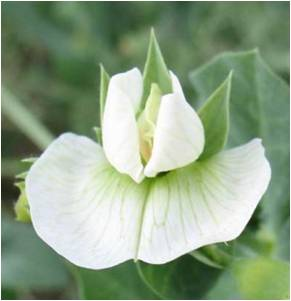
\includegraphics[width=0.60\linewidth]{./images/self_pollinated_pea.jpg}
  \end{center}
  
  \column{.2\linewidth}
  \caption{\newline \scriptsize Self pollinating crop (top: Tomato; bottom: Pea)}
  \label{fig:self-pollinating-crop}
  
  \end{columns}
\end{figure}
\end{frame}

\hypertarget{breeding-self-pollinated-crops}{%
\section{Breeding self pollinated
crops}\label{breeding-self-pollinated-crops}}

\begin{frame}{Mass selection}
\protect\hypertarget{mass-selection}{}
\begin{itemize}
\tightlist
\item
  Mass selection (originally described by Danish biologist W. Johansen,
  1903) is an example of selection from a biologically variable
  population in which differences are genetic in origin.
\item
  Often described as the oldest method of breeding self-pollinated plant
  species.
\item
  Provided that there is sufficient genetic variation, this method of
  selection is applicable to both self- and cross-pollinated species.
\item
  Common method of seed saving of best appearing plants is comparable to
  mass selection.
\item
  Major objective: Population improvement by increasing gene frequencies
  of desirable genes.
\end{itemize}
\end{frame}

\begin{frame}{}
\protect\hypertarget{section-1}{}
\begin{itemize}
\tightlist
\item
  General procedure in mass selection is to rogue out off-types or
  plants with undesirable traits (\emph{Negative mass selection}).
\item
  The specific strategies for retaining representative individuals for
  the population vary according to species, traits of interest, or
  creativity of the breeder.
\item
  Rouging out and bulking appears to be the basic strategy of mass
  selection, some breeders may rather select and advance a large number
  of plants that are desirable and uniform for the trait(s) of interest
  (\emph{positive mass selection}).
\item
  Where applicable, single pods from each plant may be picked and bulked
  for planting. For cereal species, the heads may be picked and bulked.
\end{itemize}
\end{frame}

\begin{frame}{}
\protect\hypertarget{section-2}{}
\begin{figure}

{\centering 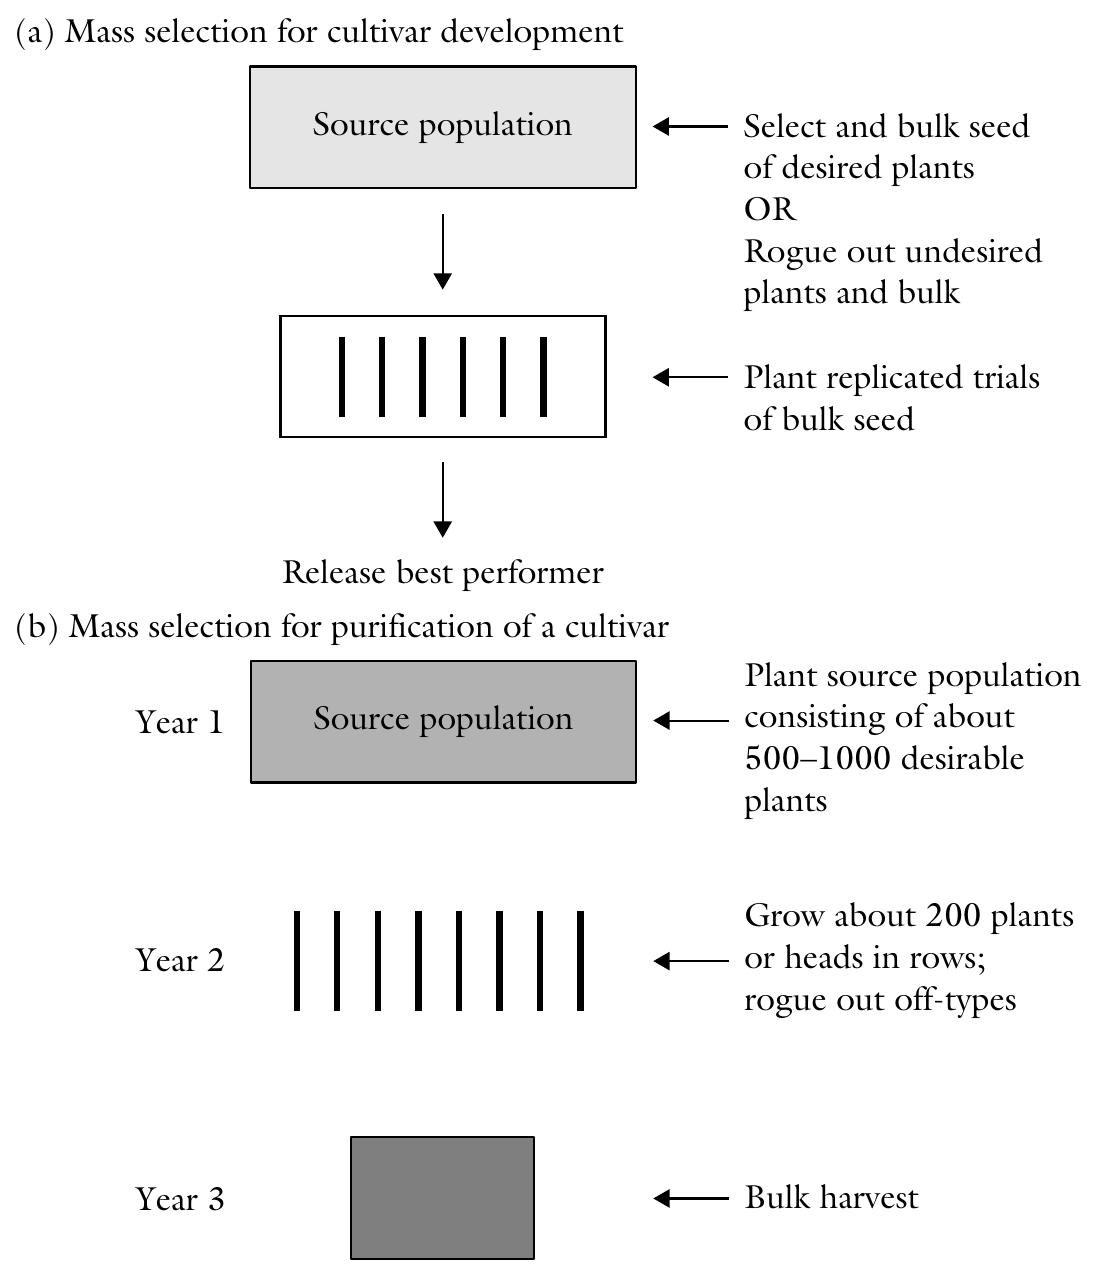
\includegraphics[width=0.55\linewidth]{./images/mass_selection} 

}

\caption{Mass selection in self pollinated crops}\label{fig:mass-selection}
\end{figure}
\end{frame}

\begin{frame}{}
\protect\hypertarget{section-3}{}
\begin{itemize}
\tightlist
\item
  The breeder plants the heterogeneous population in the field, looks
  for off-types to remove and discard.
\item
  A mechanical device (e.g., using a sieve to determine which size of
  grain would be advanced) may be used, or selection may be purely on
  visual basis according to the breeder's visual evaluation.
\item
  Further, selection may be based on targeted traits (\emph{direct
  selection}) or indirectly by selecting a trait correlated with the
  trait to be improved.

  \begin{itemize}
  \tightlist
  \item
    Year 1: If the objective is to purify an established cultivar, seed
    of selected plants may be progeny rowed to confirm the purity of the
    selected plants prior to bulking. This would make a cycle of mass
    selection have a two-year duration instead of one year. The original
    cultivar needs to be planted alongside for comparison.
  \item
    Year 2: Evaluate composite seed in replicated trial, using original
    cultivar as check. This test may be conducted at different locations
    and over several years. The seed is bulk-harvested.
  \end{itemize}
\end{itemize}
\end{frame}

\begin{frame}{}
\protect\hypertarget{section-4}{}
\begin{itemize}
\tightlist
\item
  Contamination from outcrossing may produce heterozygotes in the
  population. Mass selection is most effective if the expression of the
  trait of interest is conditioned by additive gene action.
\item
  With Masss selection,

  \begin{itemize}
  \tightlist
  \item
    In self-pollinated populations, the persistence of inbreeding will
    alter population gene frequencies by reducing heterozygosity from
    one generation to the next.
  \item
    In cross-pollinated populations, gene frequencies are expected to
    remain unchanged unless the selection ofplants was biased enough to
    change the frequency of alleles that control the trait of interest.
  \item
    Mass selection is based on plant phenotype. Consequently, it is most
    effective if the trait of interest has high heritability.
  \end{itemize}
\item
  Selection is effective when environment is uniform. For example, When
  selecting for disease resistance, the method is more effective if the
  pathogen is uniformly present throughout the field without ``hot
  spots''.
\item
  Correlated response to selection for secondary traits.
\end{itemize}
\end{frame}

\begin{frame}{Advantages}
\protect\hypertarget{advantages}{}
\begin{itemize}
\tightlist
\item
  It is rapid, simple, and straightforward. Large populations can be
  handled and one generation per cycle can be used.
\item
  It is inexpensive to conduct.
\item
  The cultivar is phenotypically fairly uniform even though it is a
  mixture of pure lines.
\end{itemize}
\end{frame}

\begin{frame}{Disadvantages}
\protect\hypertarget{disadvantages}{}
\begin{itemize}
\tightlist
\item
  To be most effective, the traits of interest should have high
  heritability.
\item
  Because selection is based on phenotypic values, optimal selection is
  achieved if it is conducted in a uniform environment.
\item
  Phenotypic uniformity is less than in cultivars produced by pure line
  selection.
\item
  With dominance, heterozygotes are indistinguishable from homozygous
  dominant genotypes. Without progeny testing, the selected
  heterozygotes will segregate in the next generation.
\end{itemize}
\end{frame}

\hypertarget{pure-line-selection}{%
\section{Pure line selection}\label{pure-line-selection}}

\begin{frame}{}
\protect\hypertarget{section-5}{}
\bcolumns
\column{0.35\textwidth}

\begin{itemize}
\tightlist
\item
  A pure line suggests that a cultivar has
  \alert{identical alleles at all loci}.
\item
  The theory was developed in 1903 by the Danish botanist Johannsen.
\end{itemize}

\column{0.65\textwidth}
\begin{figure}

{\centering 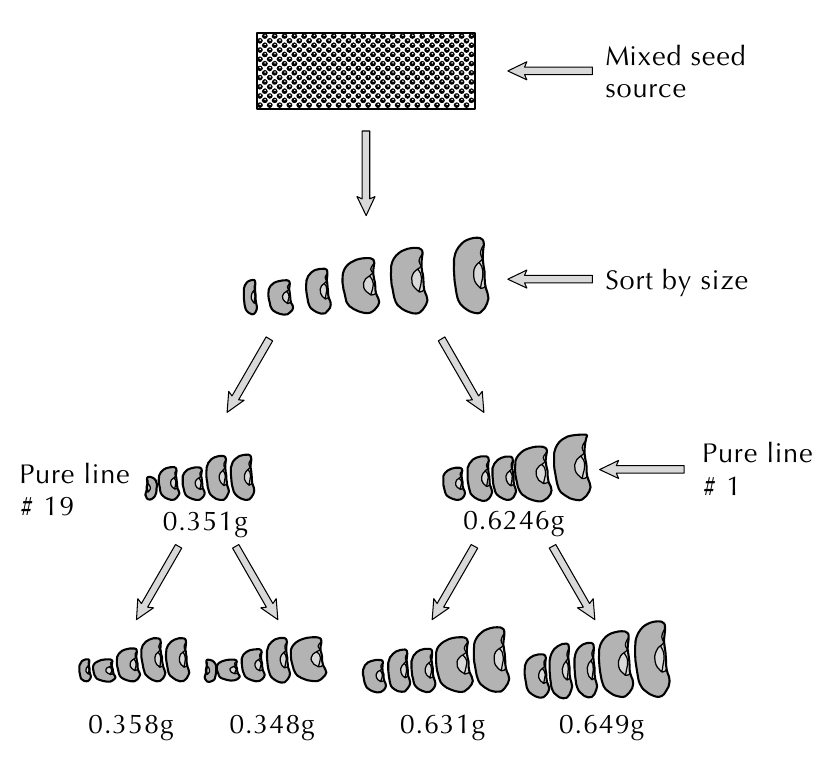
\includegraphics[width=0.75\linewidth]{./images/johannsen_bean} 

}

\caption{The development of the pure line theory by Johannsen}\label{fig:johannsen-bean}
\end{figure}

\ecolumns
\end{frame}

\begin{frame}{}
\protect\hypertarget{section-6}{}
\begin{itemize}
\tightlist
\item
  Johannsen demonstrated that a mixed population of self-pollinated
  species could be sorted out into genetically pure lines.
\item
  These lines were subsequently non-responsive to selection within each
  of them .
\item
  Selection is a passive process, since it eliminates variation but does
  not create it.
\item
  Lines that are genetically different may be successfully isolated from
  within a population of mixed genetic types.
\item
  Any variation that occurs within a pure line is not heritable but due
  to environmental factors only. Consequently, as Johansen's bean study
  showed, further selection within the line is not effective.
\item
  Lines are used;

  \begin{itemize}
  \tightlist
  \item
    as cultivars or as parents in hybrid production (inbred lines).
  \item
    in the development of genetic stock (containing specific genes such
    as disease resistance, nutritional quality) and synthetic and
    multiline cultivars.
  \end{itemize}
\item
  Line cultivars have a very narrow genetic base and tend to be uniform
  in traits of interest (e.g., height, maturity).
\end{itemize}
\end{frame}

\begin{frame}{Application}
\protect\hypertarget{application}{}
\begin{itemize}
\tightlist
\item
  Cultivars for mechanized production that must meet a certain
  specification for uniform operation by farm machines (e.g., uniform
  maturity, uniform height for uniform location of economic part).
\item
  Cultivars developed for a discriminating market that puts a premium on
  eye-appeal (e.g., uniform shape, size).
\item
  Cultivars for the processing market (e.g., with demand for certain
  canning qualities, texture).
\item
  Advancing ``sports'' that appear in a population (e.g., a mutant
  flower for ornamental use).
\item
  Improving newly domesticated crops that have some variability.
\item
  The pure-line selection method is also an integral part of other
  breeding method,s such as the pedigree selection and bulk population
  selection.
\end{itemize}
\end{frame}

\begin{frame}{Overview}
\protect\hypertarget{overview}{}
\begin{itemize}
\tightlist
\item
  The pure-line selection in breeding entails repeated cycles of selfing
  following the initial selection from a mixture of homozygous lines.
\item
  Natural populations of self-pollinated species consist of mixtures of
  homozygous lines with transient heterozygosity originating from
  mutations and outcrossing.
\item
  Steps:

  \begin{itemize}
  \tightlist
  \item
    Year 1: The first step is to obtain a variable base population
    (e.g., introductions, segregating populations from crosses, land
    race) and space plant it in the first year, select, and harvest
    desirable individuals.
  \item
    Year 2: Grow progeny rows of selected plants. Rogue out any
    variants. Harvest selected progenies individually. These are
    experimental strains.
  \item
    Year 3-6: Conduct preliminary yield trials of the experimental
    strains including appropriate check cultivars.
  \item
    Year 7-10: Conduct advanced yield trials at multilocations. Release
    highest yielding line as new cultivar.
  \end{itemize}
\end{itemize}
\end{frame}

\begin{frame}{}
\protect\hypertarget{section-7}{}
\begin{figure}

{\centering 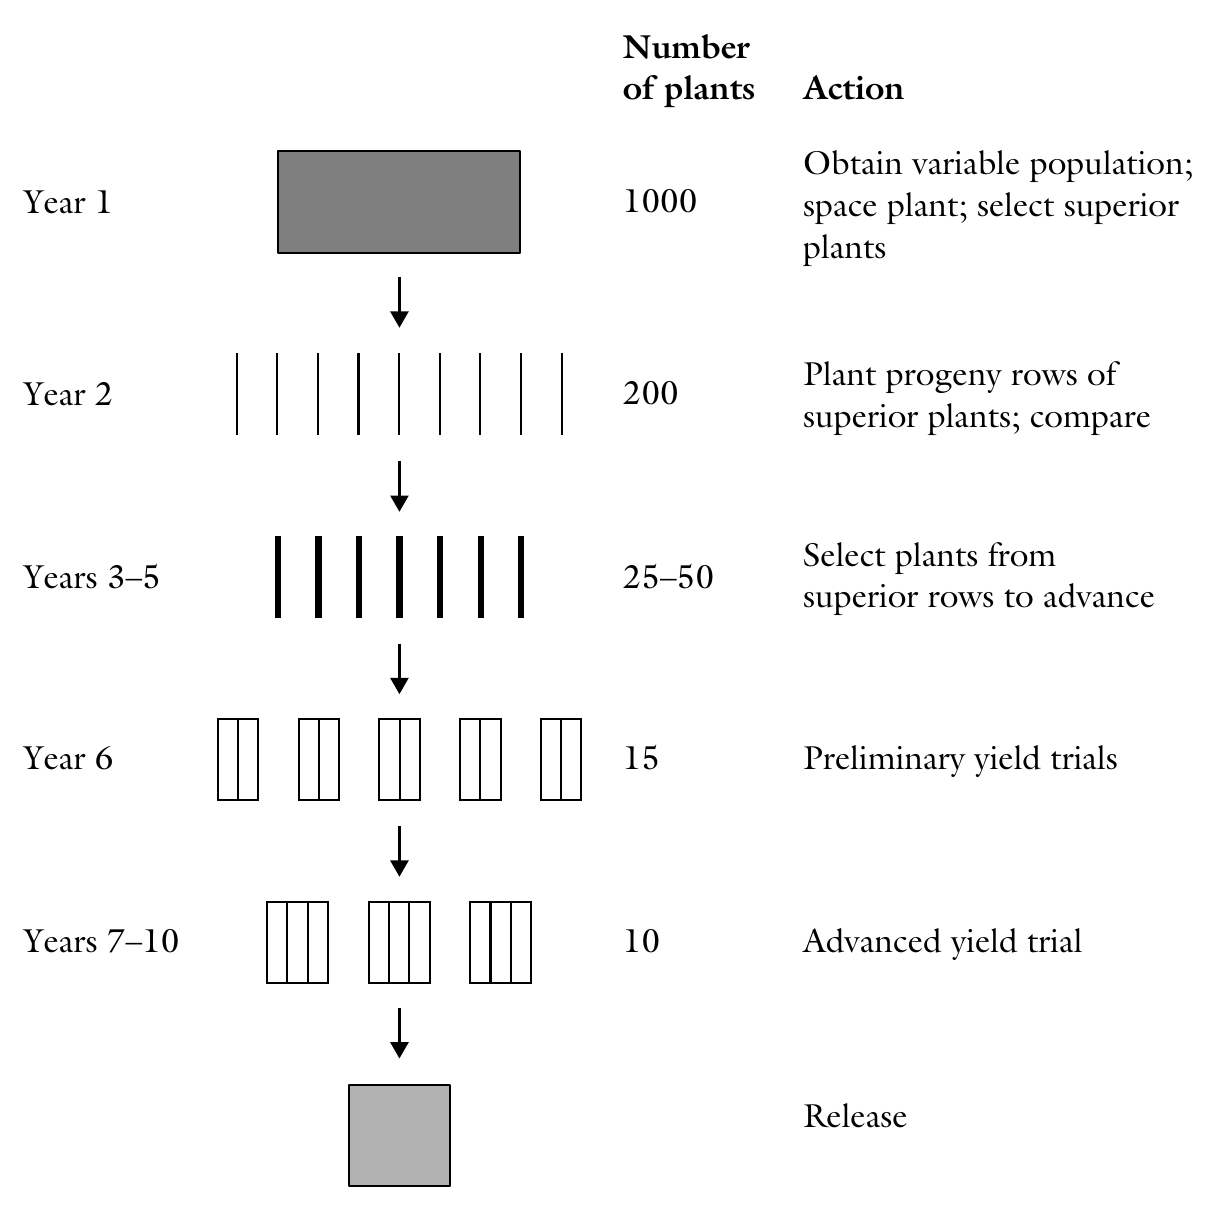
\includegraphics[width=0.56\linewidth]{./images/pureline_selection} 

}

\caption{Generalized steps in breeding by pure-line selection}\label{fig:pureline-selection}
\end{figure}
\end{frame}

\begin{frame}{Genetic issues of pureline selection}
\protect\hypertarget{genetic-issues-of-pureline-selection}{}
\begin{itemize}
\tightlist
\item
  Pure-line breeding produces cultivars with a narrow genetic base and,
  hence, that are less likely to produce stable yields over a wider
  range of environments. Such cultivars are more prone to being wiped
  out by pathogenic outbreaks.
\item
  Pure-line cultivars depend primarily on phenotypic plasticity for
  production response and stability across environments.
\end{itemize}
\end{frame}

\begin{frame}{Advantages}
\protect\hypertarget{advantages-1}{}
\begin{itemize}
\tightlist
\item
  It is a rapid breeding method.
\item
  The method is inexpensive to conduct. The base population can be a
  landrace. The population size selected is variable and can be small or
  large, depending on the objective.
\item
  The cultivar developed by this method has great ``eye appeal''
  (because of the high uniformity of, e.g., harvesting time, height,
  etc.).
\end{itemize}
\end{frame}

\begin{frame}{Disadvantages}
\protect\hypertarget{disadvantages-1}{}
\begin{itemize}
\tightlist
\item
  The purity of the cultivar may be altered through admixture, natural
  crossing with other cultivars, and mutations. Such off-type plants
  should be rogued out to maintain cultivar purity.
\item
  The cultivar has a narrow genetic base and, hence, is susceptible to
  devastation from adverse environmental factors because of uniform
  response.
\item
  A new genotype is not created. Rather, improvement is limited to the
  isolation of the most desirable or best genotype from a mixed
  population.
\item
  The method promotes genetic erosion because most superior pure lines
  are identified and multiplied to the exclusion of other genetic
  variants.
\item
  Progeny rows takes up more resources (time, space, funds).
\end{itemize}
\end{frame}

\hypertarget{pedigree-selection}{%
\section{Pedigree selection}\label{pedigree-selection}}

\begin{frame}{}
\protect\hypertarget{section-8}{}
\begin{figure}

{\centering 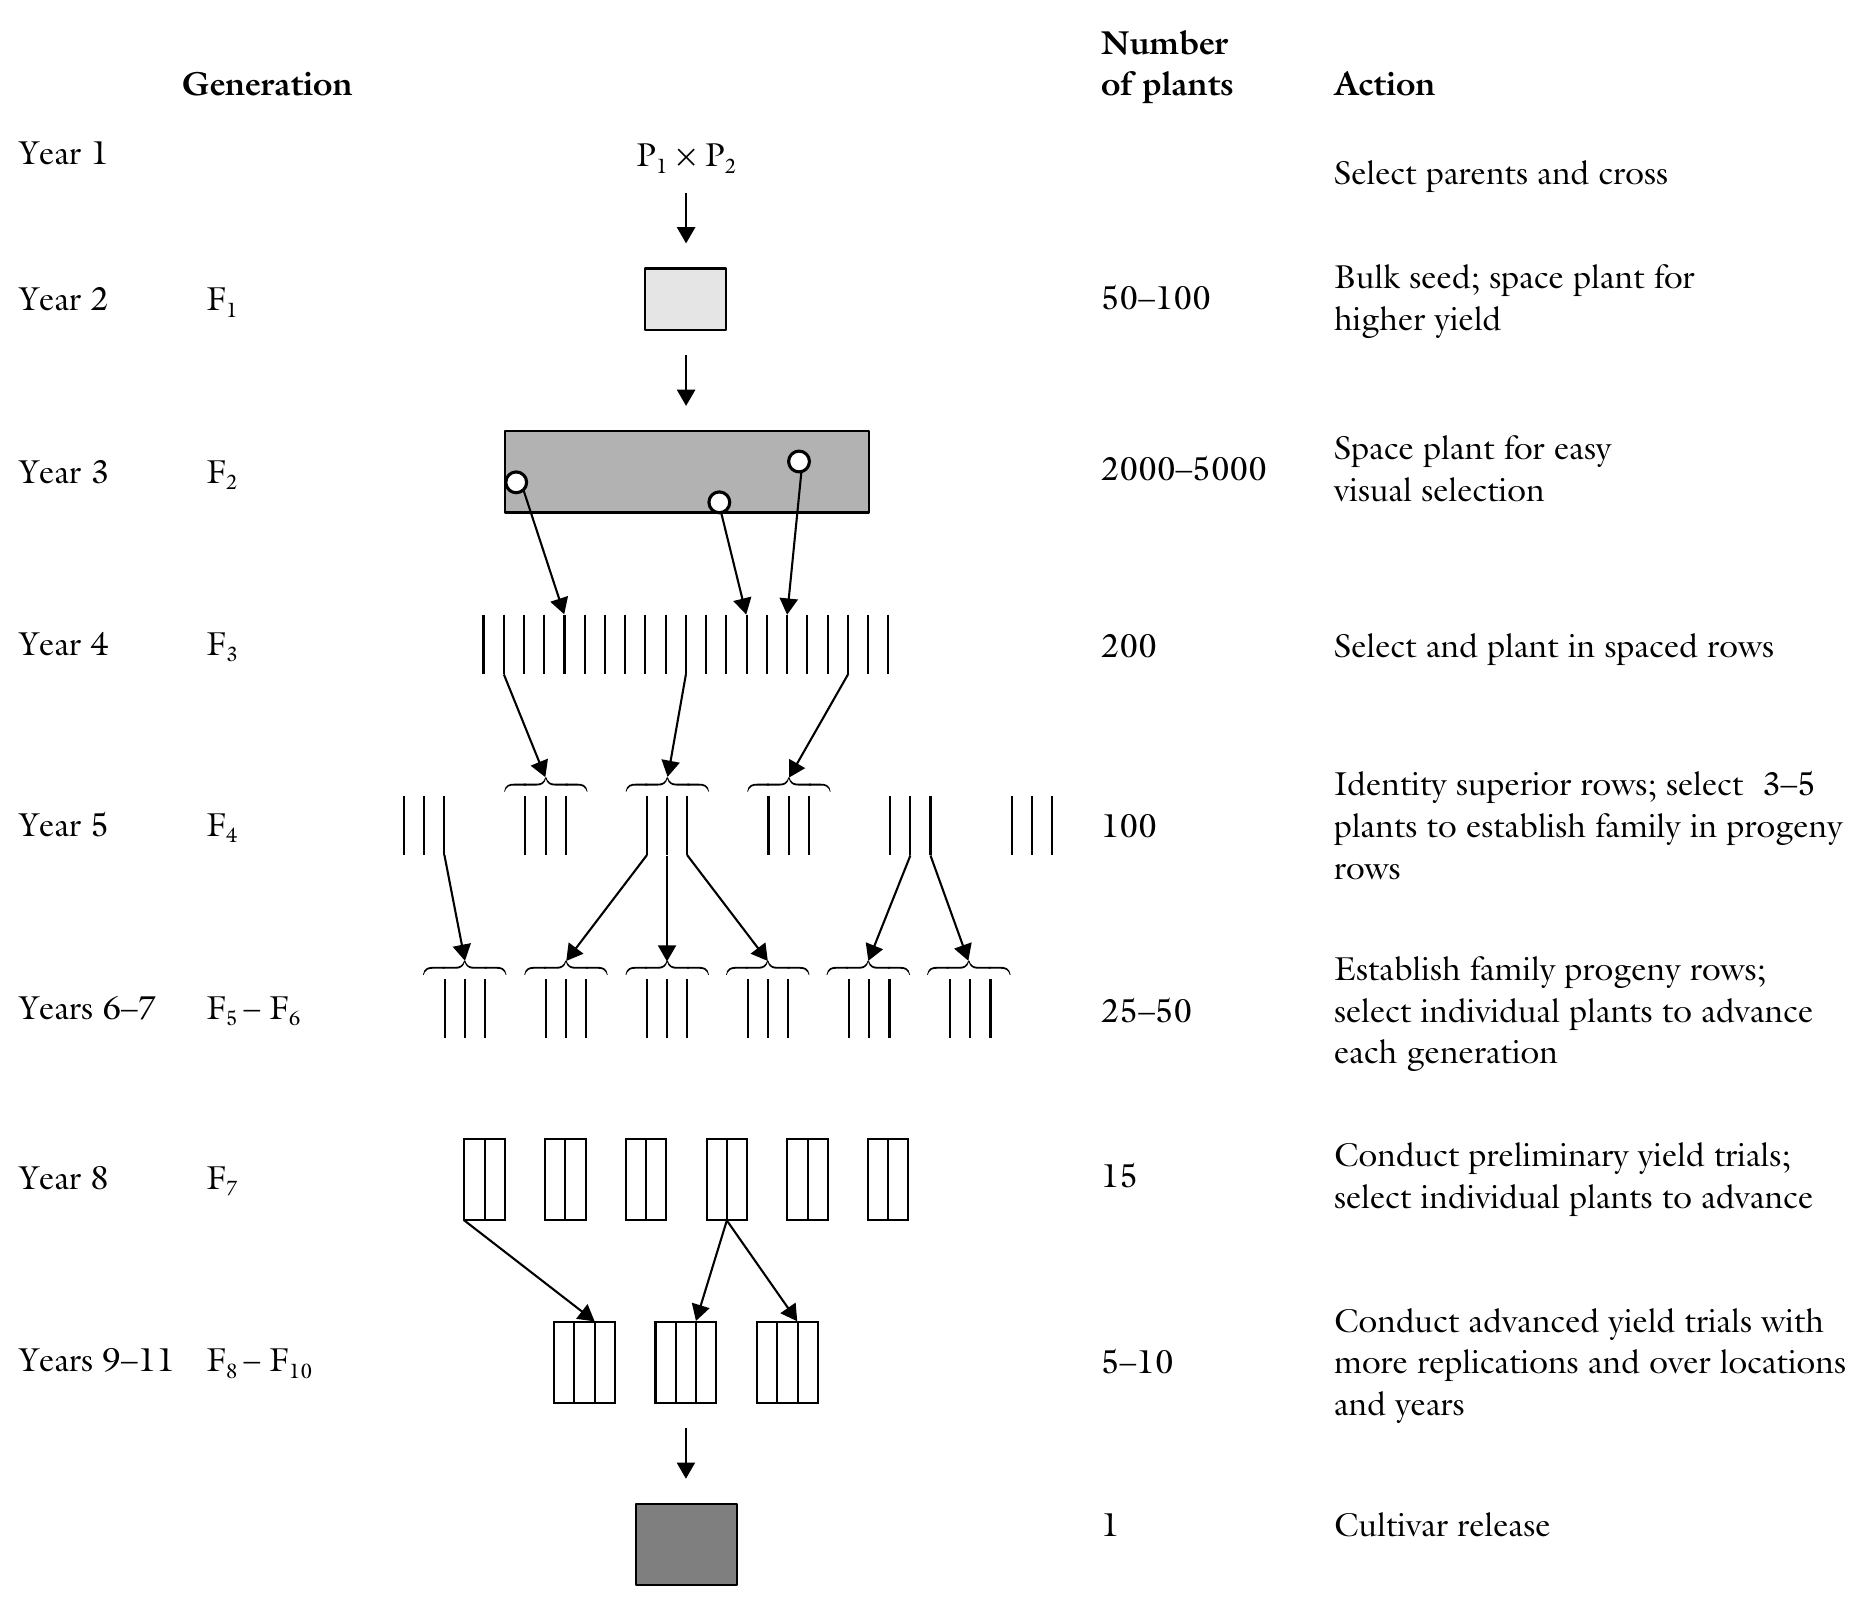
\includegraphics[width=0.64\linewidth]{./images/pedigree_selection} 

}

\caption{Generalized steps in breeding by pedigree selection}\label{fig:pedigree-selection}
\end{figure}
\end{frame}

\hypertarget{bulk-population}{%
\section{Bulk population}\label{bulk-population}}

\begin{frame}{}
\protect\hypertarget{section-9}{}
\begin{figure}

{\centering 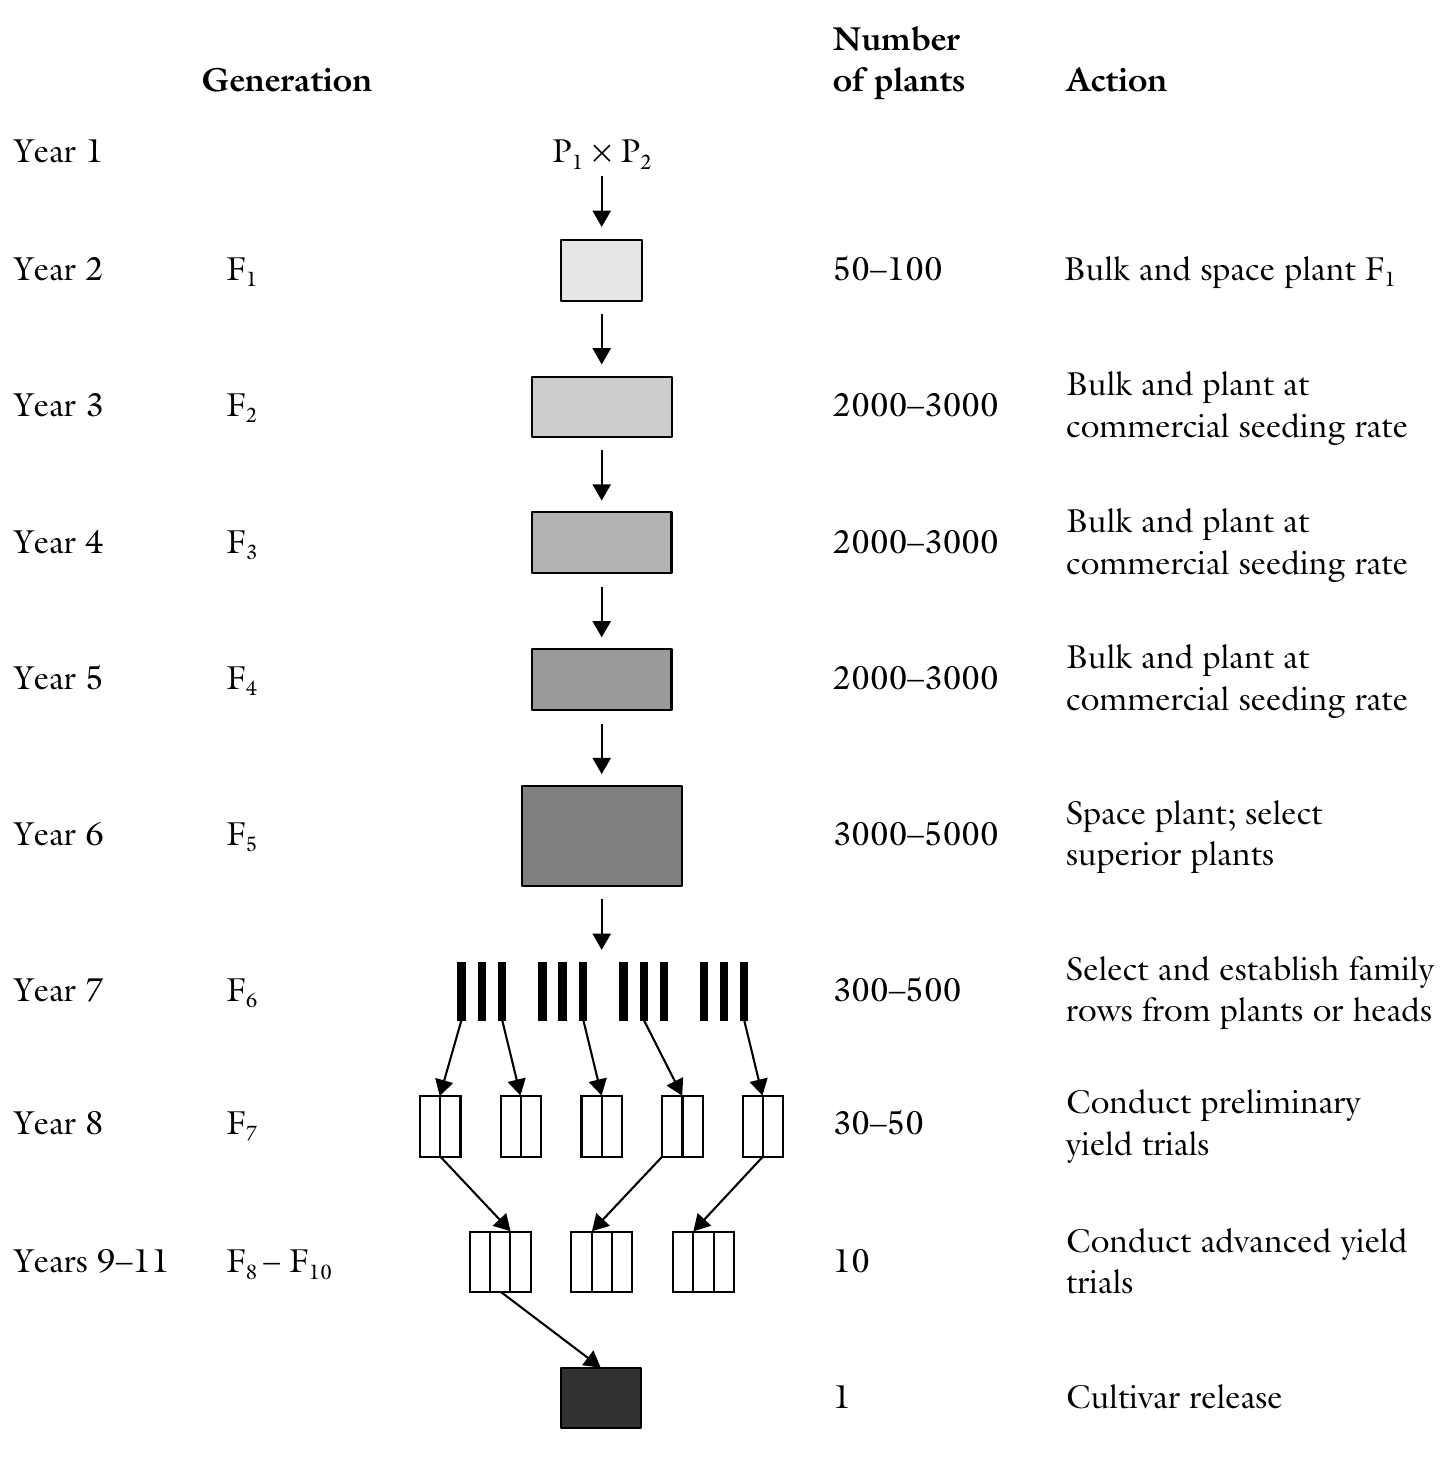
\includegraphics[width=0.56\linewidth]{./images/bulk_selection} 

}

\caption{Generalized steps in breeding by bulk selection}\label{fig:bulk-selection}
\end{figure}
\end{frame}

\hypertarget{single-seed-descent}{%
\section{Single seed descent}\label{single-seed-descent}}

\begin{frame}{}
\protect\hypertarget{section-10}{}
\begin{itemize}
\tightlist
\item
  The method of single seed descent was born out of a need to speed up
  the breeding program by rapidly inbreeding a population prior to
  beginning individual plant selection and evaluation, while reducing a
  loss of genotypes during the segregating generations.
\item
  The concept was first proposed by C.H. Goulden in 1941 when he
  attained the F6 generation in two years by reducing the number of
  generations grown from a plant to one or two, while conducting
  multiple plantings per year, using the greenhouse and the off season.
\item
  However, it was C.A. Brim who, in 1966, provided a formal description
  of the procedure of single seed descent, calling it a modified
  pedigree method.
\end{itemize}
\end{frame}

\begin{frame}{}
\protect\hypertarget{section-11}{}
\begin{itemize}
\tightlist
\item
  A large F1 population is generated to ensure adequate recombination
  among parental chromosomes.
\item
  The method allows the breeder to advance the maximum number of F2
  plants through the F5 generation.
\item
  This is achieved by advancing \emph{one} randomly selected seed per
  plant through the early segregating stages.
\item
  The focus on the early stages of the procedure is on attaining
  homozygosity as rapidly as possible, without selection.
\item
  Then, each plant is used to establish a family to help breeders in
  selection and to increase seed for subsequent yield trails.
\item
  Discriminating among plants starts after attainment of homozygosity.
\end{itemize}
\end{frame}

\begin{frame}{Steps}
\protect\hypertarget{steps}{}
\begin{itemize}
\tightlist
\item
  Year 1. Crossing is used to create the base population. Cross selected
  parents to generate adequate number of F1 for the production of a
  large F2 population.
\item
  Year 2. About 50-100 F1 plants are grown in a greenhouse ground bench
  or in pots. They may also be grown in the field. Harvest identical F1
  crosses and bulk.
\item
  Year 3. About, 2000-3000 F2 plants are grown. At maturity, a single
  seed per plant is harvested and bulked for planting F3. Subsequently,
  F2 is spaced enough to allow each plant to produce only a few seeds.
\item
  Year 4-6. Single pods per plant are harvested to plant the F4. The F5
  is space-planted in the field, harvesting seed from only superior
  plants to grow progeny rows in the F6 generation.
\item
  Year 7. Superior rows are harvested to grow preliminary yield trails
  in the F7
\item
  Year 8 and later. Yield trials are conducted in the F8 to F10
  generations. The most superior line is increased in the F11 and F12 as
  a new cultivar.
\end{itemize}
\end{frame}

\begin{frame}{Comments}
\protect\hypertarget{comments}{}
\begin{itemize}
\tightlist
\item
  If the sample is too small, superior genetic combinations may be lost
  because only one seed from each plant is used.
\item
  It may be advantageous to use progeny rows prior to yield testing to
  produce sufficient seed as well as to help in selecting superior
  families.
\item
  The breeder may choose to impose some artificial selection pressure by
  excluding undesirable plants from contributing to the subsequent
  generations (in the early generations). This is effective for
  qualitative traits.
\item
  Record keeping is minimal and so are other activities such as
  harvesting, especially in early generations.
\end{itemize}
\end{frame}

\hypertarget{backcross-breeding}{%
\section{Backcross breeding}\label{backcross-breeding}}

\begin{frame}{}
\protect\hypertarget{section-12}{}
\begin{itemize}
\tightlist
\item
  This application in plants was first proposed by H.V. Harlan and M.N.
  Pope in 1922.
\item
  The rationale of backcross breeding is to replace a specific
  undesirable gene with a desirable alternative, while preserving all
  other qualities (adaptation, productivity, etc.) of an adapted
  cultivar (or breeding line).
\item
  Instead of inbreeding the F1 as normally done, it is repeatedly
  crossed with the desirable parent to retrieve (by ``modified
  inbreeding'') the desirable genotype.
\item
  The adapted and highly desirable parent is called the \emph{recurrent
  parent} in the crossing program, while the source of the desirable
  gene missing in the adapted parent is called the \emph{donor parent}.
\item
  Even though the chief role of the donor parent is to supply the
  missing gene, it should not be significantly deficient in other
  desirable traits. An inferior recurrent parent will still be inferior
  after the gene transfer.
\end{itemize}
\end{frame}

\begin{frame}{}
\protect\hypertarget{section-13}{}
\bcolumns
\column{0.5\textwidth}

\small \textbf{Dominant gene transfer}

\begin{figure}

{\centering 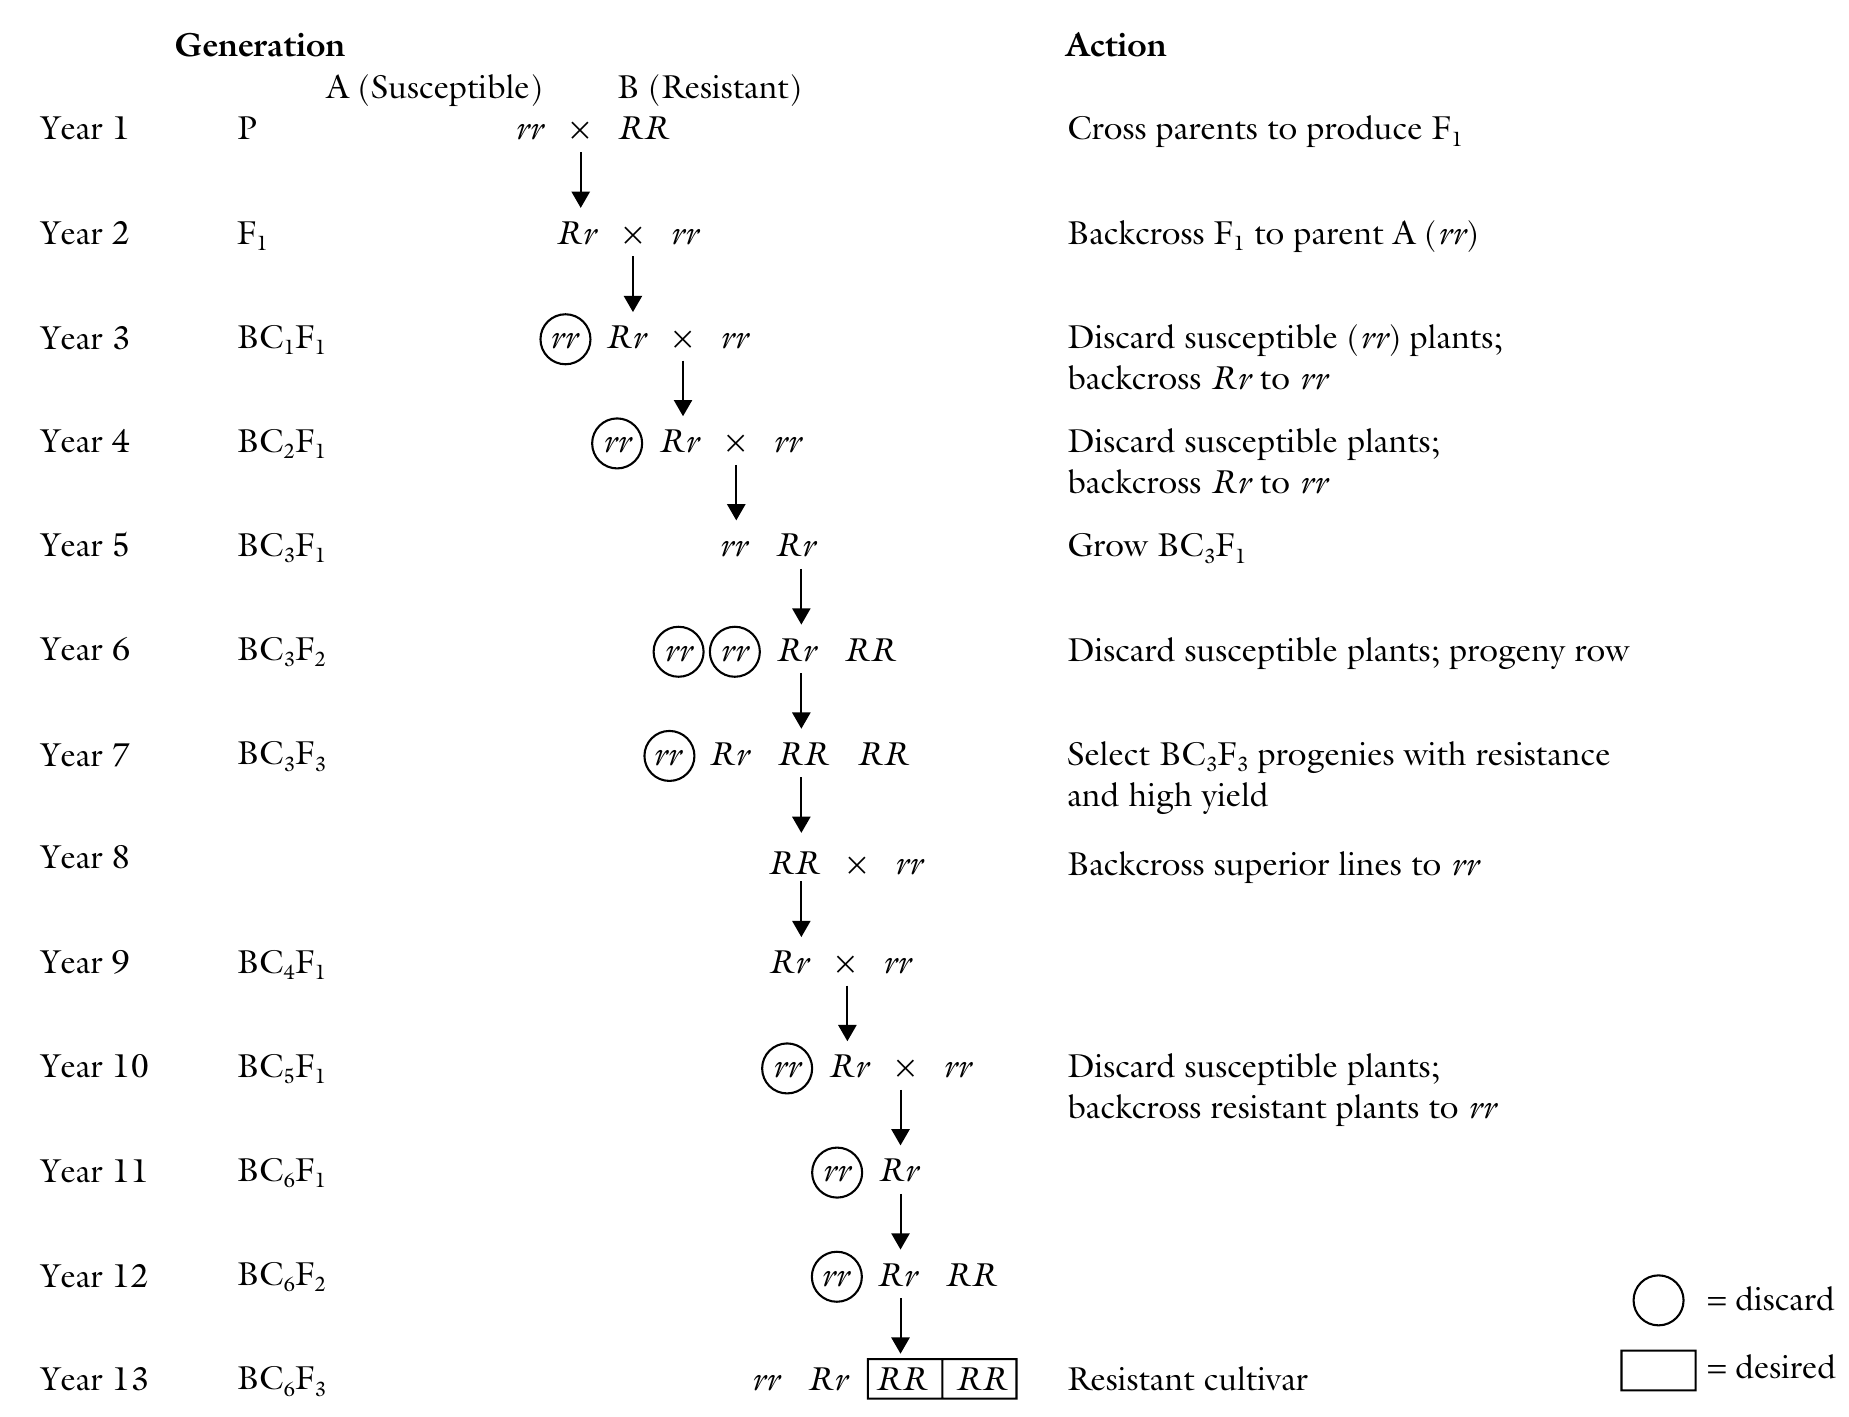
\includegraphics[width=0.85\linewidth]{./images/backcross_dominant} 

}

\caption{Generalized steps in breeding a dominant trait by the backcross method.}\label{fig:dominant-backcross-transfer}
\end{figure}

\column{0.5\textwidth}

\small \textbf{Recessive gene transfer}

\begin{figure}

{\centering 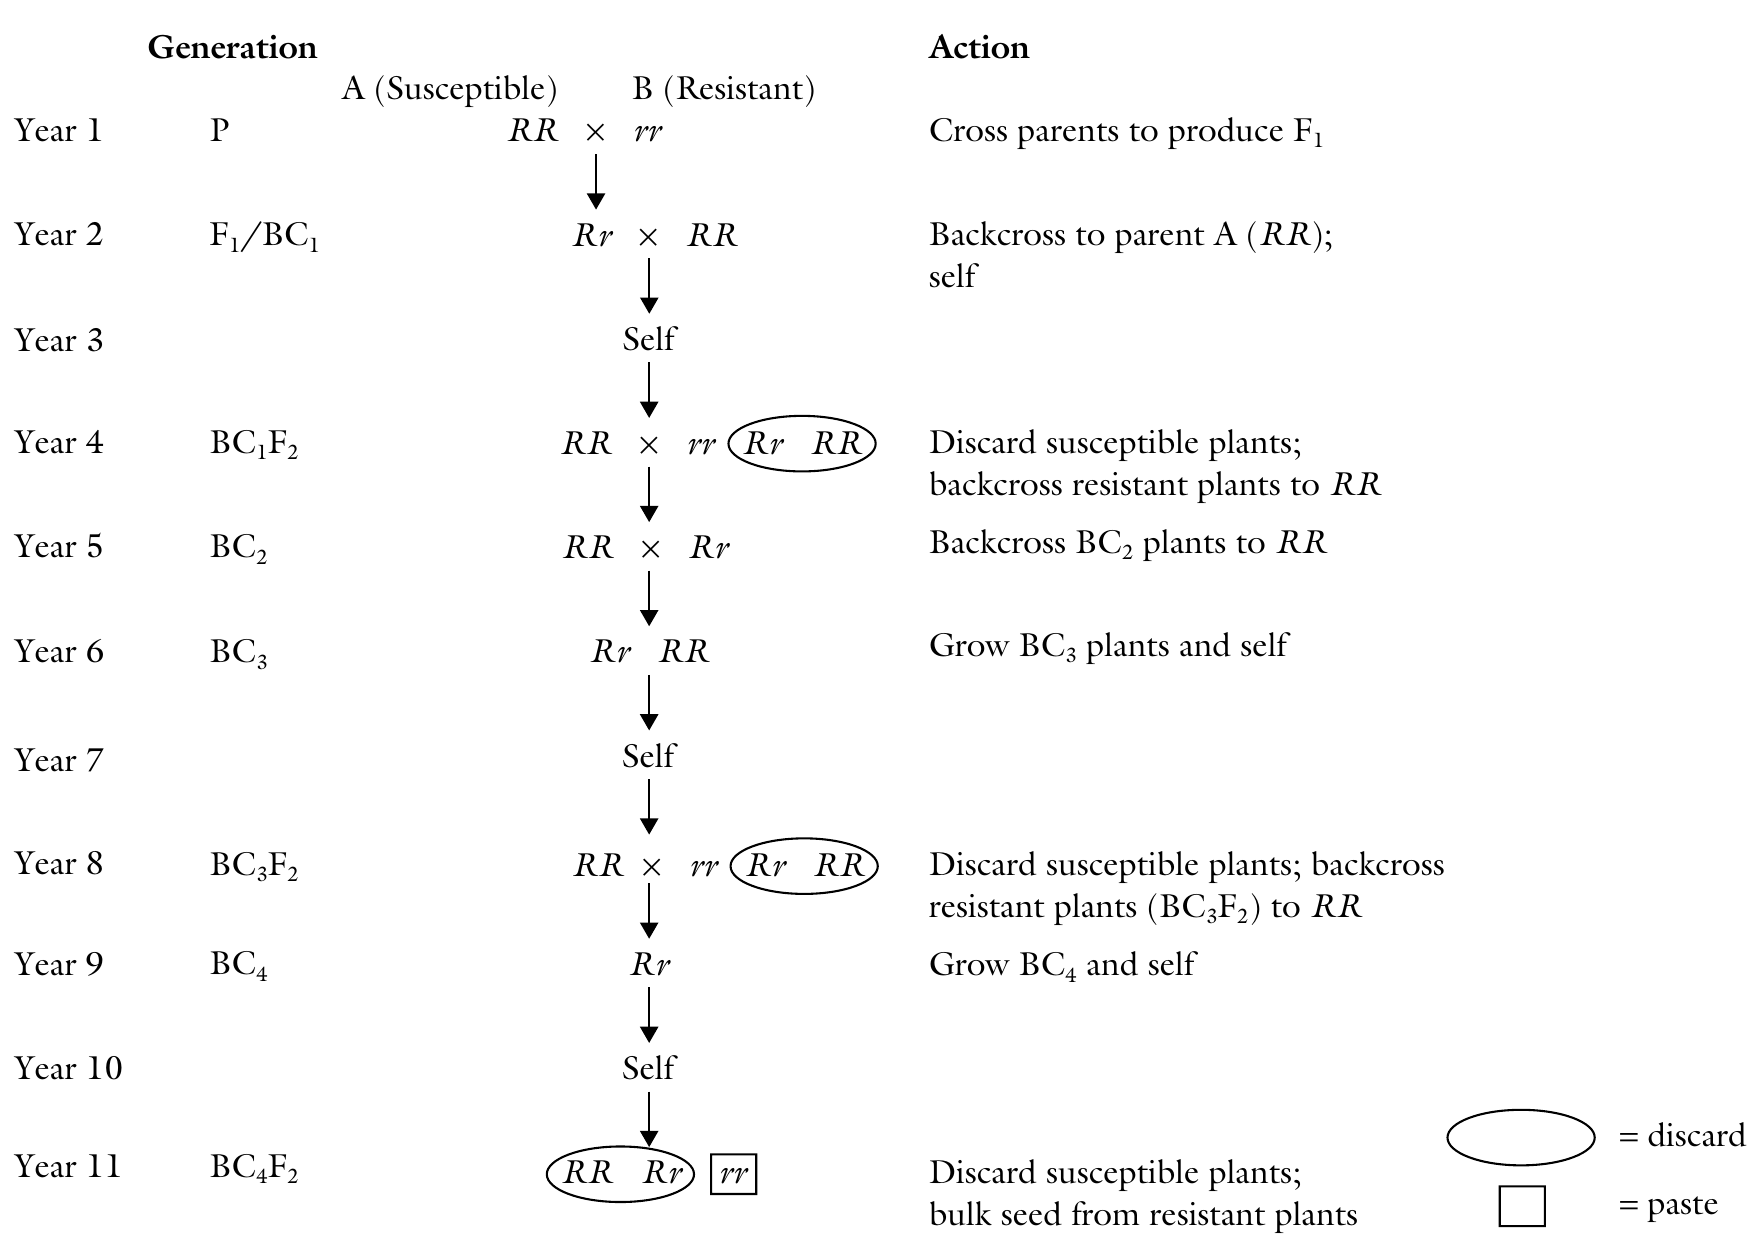
\includegraphics[width=0.85\linewidth]{./images/backcross_recessive} 

}

\caption{Generalized steps in breeding a recessive trait by the backcross method.}\label{fig:recessive-backcross-transfer}
\end{figure}

\ecolumns
\end{frame}

\begin{frame}{Genetic issues}
\protect\hypertarget{genetic-issues}{}
\begin{itemize}
\tightlist
\item
  In theory, the BC3 genotype will be 93.75\% identical to the recurrent
  parent. The mathematical relationship for the recovery of the
  recurrent parent is presented by W. Allard is:
\end{itemize}

\[
1-\left(\frac{1}{2}\right)^{m+1}
\]

where \(m\) is the number of generations of selfing or backcrosses. Same
relation also gives the proportion of homozygous individuals in any
generations of recurrent selfing. For example, for \(3^{rd}\) BC
generation,

\[
\begin{aligned}
1-\left(\frac{1}{2}\right)^{m+1} &=& 1-\left(\frac{1}{2}\right)^{3+1} \\
~ &=& 1-\left(\frac{1}{16}\right) \\
~ &=& 0.9375
\end{aligned}
\]
\end{frame}

\begin{frame}{}
\protect\hypertarget{section-14}{}
In another way, the proportion of the donor genes is reduced by 50\%
following each generation of backcrossing. This is obtained by the
relationship \(\left(\frac{1}{2}\right)^{m+1}\), where m is the number
of crosses and backcross to the parent. For example, in the BC4, the
value is \(\left(\frac{1}{2}\right)^{5} = 3.125\%\). To obtain the
percentage of homozygotes for alleles of recurrent parents in any
generation, the mathematical relationship is:

\[\left[\frac{\left(2^{m+1}\right)-1}{2^{m+1}}\right]^{n}\]

Where \(n\) is the number of genes.
\end{frame}

\begin{frame}{}
\protect\hypertarget{section-15}{}
\begin{itemize}
\tightlist
\item
  Because of cytoplasmic inheritance, it is sometimes critical which of
  the two parents is used as female.
\item
  Linkage drag, backcrossing is more effective in breaking linkages over
  selfing, especially where heritability is low for the undesirable
  trait.
\item
  For a given number of genes, certain number of individuals is needed
  for a chance to recover the desired genes in a BC program.
\item
  When the trait is governed by a dominant gene, it is easy to identify
  plants carrying the desired gene.
\item
  When the desired trait is conditioned by a recessive gene, an
  additional step is needed after each backcross to produce an F2
  generation in order to identify the recessive trait.
\end{itemize}
\end{frame}

\begin{frame}{Genetic advance in backcross breeding}
\protect\hypertarget{genetic-advance-in-backcross-breeding}{}
\begin{itemize}
\tightlist
\item
  Genetic advance depends on:

  \begin{itemize}
  \tightlist
  \item
    Heritability of the trait
  \item
    Sustainable intensity of trait expression
  \item
    Availability of selection aids
  \item
    Number of backcrosses of marker
  \end{itemize}
\end{itemize}
\end{frame}

\begin{frame}{Congruency backcross}
\protect\hypertarget{congruency-backcross}{}
\begin{itemize}
\tightlist
\item
  It is a modification of the standard backcross procedure whereby
  multiple backcrosses, alternating between the two parents in the cross
  (instead of restricted to the recurrent parent), are used.
\item
  The technique has been used to overcome the interspecific
  hybridization barrier of hybrid sterility, genotypic incompatibility,
  and embryo abortion that occurs in simple interspecific crosses.
\end{itemize}
\end{frame}

\begin{frame}{Some inquiries about backcross breeding method (dominant
gene)}
\protect\hypertarget{some-inquiries-about-backcross-breeding-method-dominant-gene}{}
\begin{enumerate}
\tightlist
\item
  Why selection is not done on generations prior to \(BC_3\) ?
\end{enumerate}

\begin{itemize}
\tightlist
\item
  Because recurrent parents genotype will not have been adequately fixed
  or introgressed and selection may not effectively discriminate useful
  (high yield, adapted) genotypes.
\end{itemize}

\begin{enumerate}
\setcounter{enumi}{1}
\tightlist
\item
  Why selection for lines in BC breeding not be delayed after \(BC_3\)
  or further?
\end{enumerate}

\begin{itemize}
\tightlist
\item
  Because adequate material will have been achieved and progressing to
  lower generations without selecting will add to the cost of
  maintaining large amount of germplasm.
\end{itemize}

\begin{enumerate}
\setcounter{enumi}{2}
\tightlist
\item
  Why selection should be preceded by progeny testing ?
\end{enumerate}

\begin{itemize}
\tightlist
\item
  In Self pollinated species, population structure promotes highly
  homozygous individuals. So without progeny testing, selecting for
  heterozygous individuals will not reflect true population structure.
  Selection is best carried out in homozygous individuals.
\end{itemize}
\end{frame}

\begin{frame}
\begin{enumerate}
\setcounter{enumi}{3}
\tightlist
\item
  Why not backcross in \(5^{th}\) year (again) ?
\end{enumerate}

\begin{itemize}
\tightlist
\item
  Because progeny testing should be done here to enable selection as
  early as possible.
\end{itemize}

\begin{enumerate}
\setcounter{enumi}{4}
\tightlist
\item
  Why ``RR x rr'' cross of \(8^{th}\) year is called backcross ?
\end{enumerate}

\begin{itemize}
\tightlist
\item
  Normally heterozygote when crossed with either parent is called
  backcross. In \(8^{th}\) generation, ``RR'' is crossed to the
  recurrent parent. Note, however, that ``RR'' is not fully homozygous
  for all other loci.
\end{itemize}
\end{frame}

          \begin{frame}[allowframebreaks]{}
    \bibliographytrue
    \bibliography{../bibliographies.bib}
    \end{frame}
  


\end{document}
